\documentclass[12pt]{beamer}
\usetheme{Pittsburgh}
\usecolortheme{seagull}
\usepackage[utf8]{inputenc}
\usepackage[english]{babel}
\usepackage{amsmath}
\usepackage{amsfonts}
\usepackage{amssymb}
\usepackage{graphicx}
\author{Design and Verification of Security Protocols and Security Ceremonies}
\title{\vspace{-.7cm}Cryptographic Primitives \\\vspace{-.7cm} Symmetric Cryptography}
%\setbeamercovered{transparent} 
\setbeamertemplate{navigation symbols}{} 
%\logo{
\includegraphics[scale=0.015]{Brasao_UFSC.png}
\includegraphics[scale=0.2]{brasao_PPGCC.jpg}} 
\institute{Programa de Pós-Graduacão em Ciências da Computacão \\ Dr. Jean Everson Martina} 
\date{\vspace{-1cm}August-November 2016} 
\subject{} 
\usebackgroundtemplate{
\includegraphics[width=\paperwidth,
height=\paperheight]{../reusable_images/fundo_UFSC.png}}
\begin{document}

{
\usebackgroundtemplate{
\includegraphics[width=\paperwidth,
height=\paperheight]{../reusable_images/fundo_capa.png}}
\begin{frame}
\titlepage

\includegraphics[scale=0.3]{../reusable_images/brasao_PPGCC.jpg}
\end{frame}
}

\begin{frame}{Cryptography Aims}
\begin{columns}
\column{.5\textwidth}
\begin{itemize}
\item To provide confidentiality;\pause
\item Securely exchange information in an insecure environment;\pause
\item Only valid users know how to perform decryption.\pause
\end{itemize}
\column{.5\textwidth}
\begin{center}
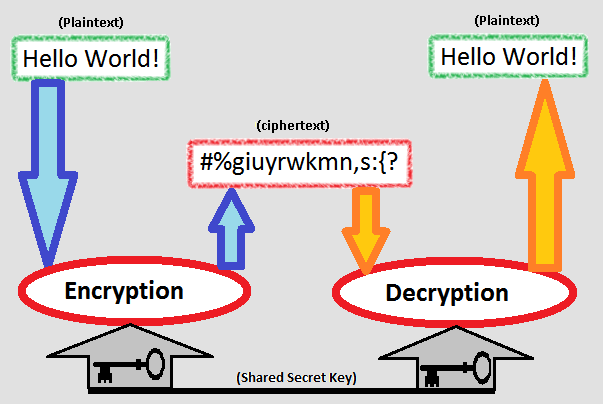
\includegraphics[scale=.35]{crypto.png}
\end{center}
\end{columns}
\end{frame}


\begin{frame}{Symmetric Cryptography Setting}
\begin{itemize}
\item Encryption and Decryption are specified algorithms;\pause
\item Two approaches:\pause
\begin{itemize}
\item Keep encryption and decryption algorithms secret: \textit{''security through
obscurity"};\pause
\item Add another variable, called a \textit{key} that must be known to encrypt and
decrypt a message;\pause
\end{itemize}
\item Symmetric-key cryptography uses same key used for both encryption and decryption.
\end{itemize}
\end{frame}


\begin{frame}{Symmetric Cryptography Problem}
\begin{itemize}
\item Symmetric-key cryptography requires the recipient of an encrypted message knows the key;\pause
\item We can not send key in a separate message because:\pause
\begin{itemize}
\item If unencrypted an adversary could intercept it and learn the key;\pause
\item If encrypted message, it would require a key that had to be distributed somehow;\pause
\end{itemize} 
\item We usually assume the key is known;\pause
\item We will talk about key distribution protocols in the next lectures.
\end{itemize}
\end{frame}

{
\usebackgroundtemplate{
\includegraphics[width=\paperwidth,
height=\paperheight]{../reusable_images/fundo_capa.png}}
\begin{frame}

{\LARGE Questions????}

\end{frame}
}

{
\usebackgroundtemplate{
\includegraphics[width=\paperwidth,
height=\paperheight]{../reusable_images/fundo_capa.png}}
\begin{frame}

\includegraphics[scale=0.8]{../reusable_images/cc_logo_arge.png}\hspace{0.5cm} 

\includegraphics[scale=0.95]{../reusable_images/by.png}

\vspace{1cm}
This work is licensed under the Creative Commons Attribution 4.0 International License. To view a copy of this license, visit http://creativecommons.org/licenses/by/4.0/.
\end{frame}
}

\end{document}